% Условная компиляция для самостоятельной работы
\ifdefined\mainfile
    % Если это часть основного файла, не добавляем начало и конец документа
\else
    \documentclass[12pt, a4paper]{report}
    \usepackage{/Users/vladbelousov/Desktop/Semestr_4-FP-NSU/Настройка/library}
    \usepackage[utf8]{inputenc} % Подключение поддержки UTF-8
    \begin{document}
\fi

%%-------------------------------%%

Вспомним \textbf{Определение 1.} 

Функция \( V (\vec{y }  ) \), определенная  в шаре  \( \underbrace{ \{\left\lVert \vec{y }   \right\rVert < r\}}_{\Leftrightarrow  y_1 ^2 + ... + y_n ^2 < r ^2 } \), называется функцией Ляпунова для системы (1) если: 

1) \( V (\vec{y } ) \in  C^1 (\left\lVert \vec{y }  \right\rVert < r ) \) 

2) \( V (\vec{y }  ) > 0 \text{ }  \forall 0 < \left\lVert  \vec{ y}  (t) \right\rVert < r , \text{ }  V(\vec{ 0 } ) =0  \) 

3) \( (\nabla V(\vec{y } ) , \vec{f } (\vec{y } ) ) \le  0 , \text{  }  \left\lVert \vec{y }  \right\rVert < r\)

\( 1) , 2) \Rightarrow  \) 

\begin{center}
    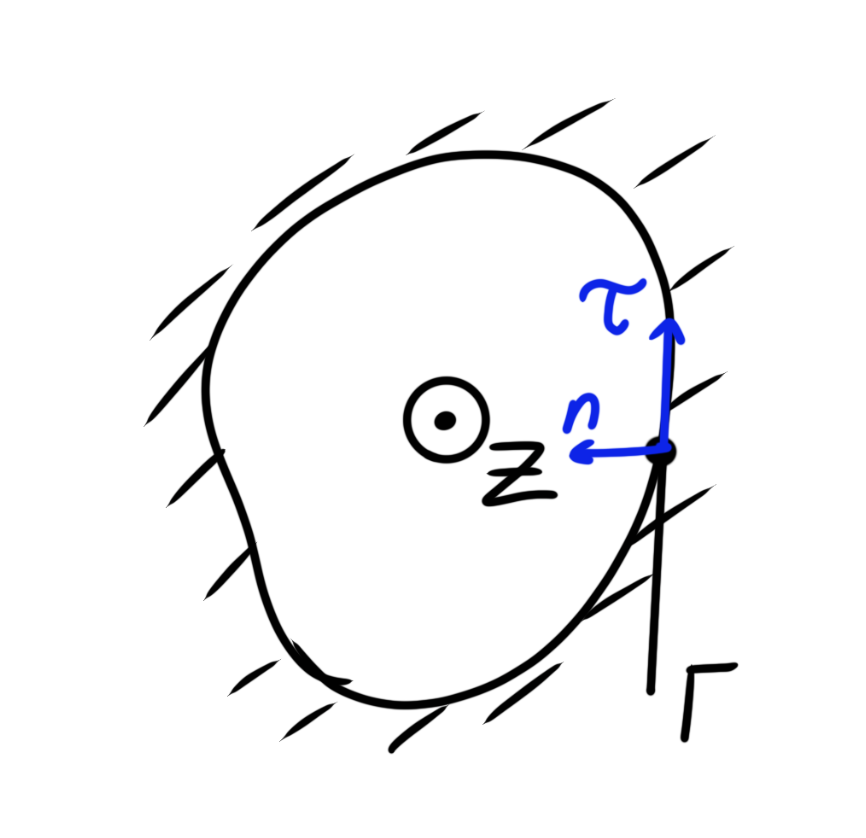
\includegraphics[width=0.4\textwidth]{/Users/vladbelousov/Desktop/Semestr_4-FP-NSU/ДфУ/Лекции_по_дням/image/54.png}
    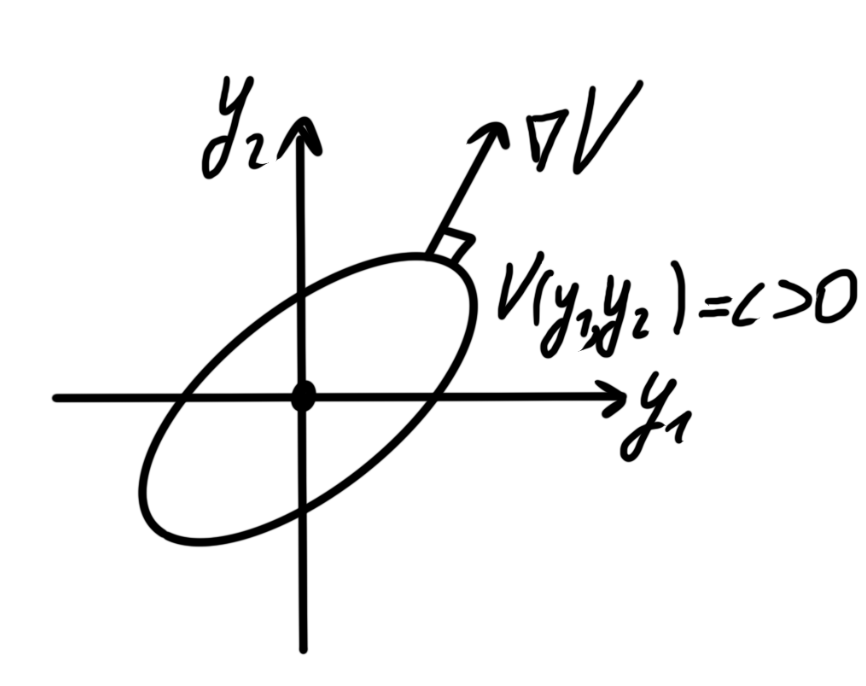
\includegraphics[width=0.4\textwidth]{/Users/vladbelousov/Desktop/Semestr_4-FP-NSU/ДфУ/Лекции_по_дням/image/55.png}
\end{center} 

\( 3) \Rightarrow \) 

\begin{center}
    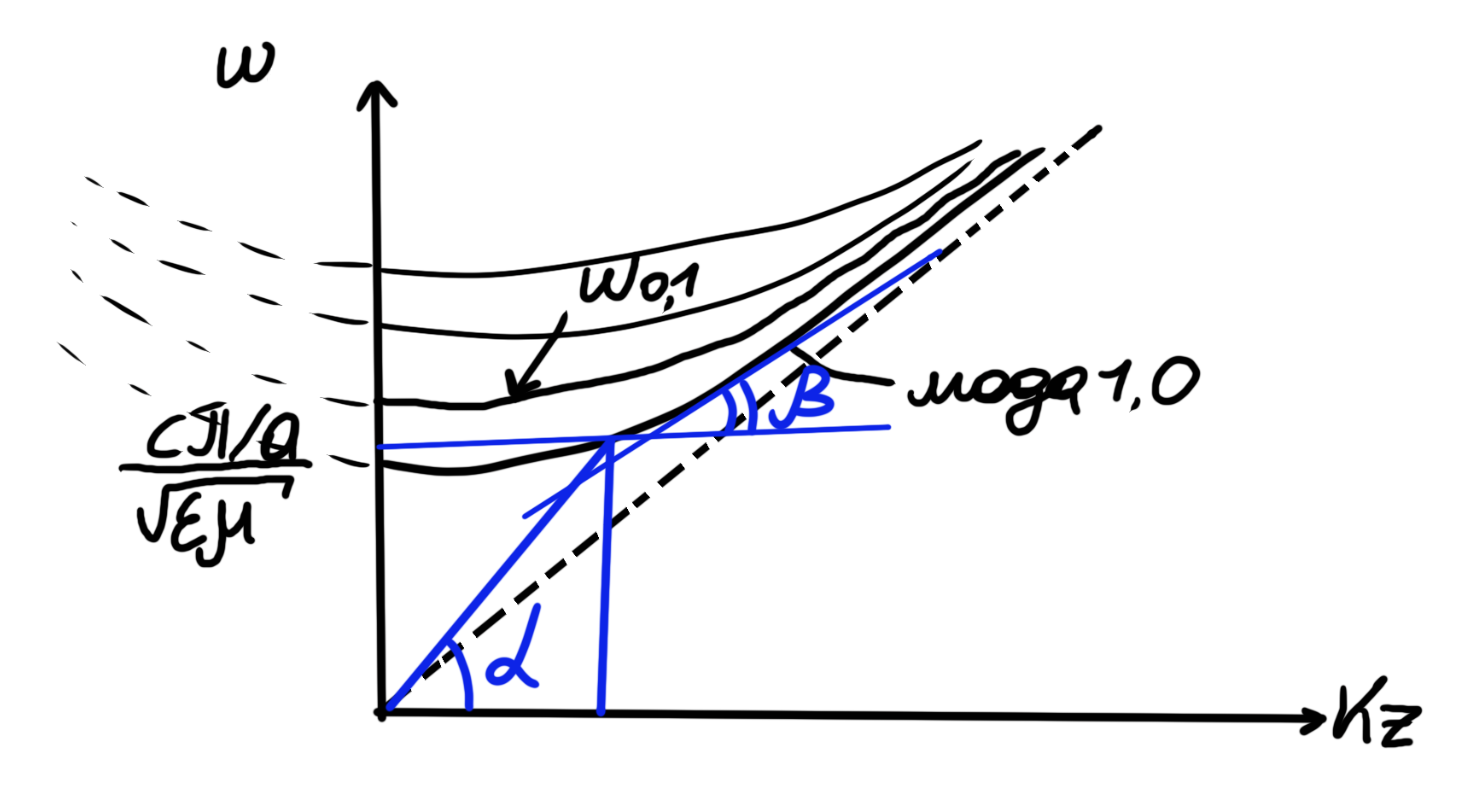
\includegraphics[width=0.6\textwidth]{/Users/vladbelousov/Desktop/Semestr_4-FP-NSU/ДфУ/Лекции_по_дням/image/56.png}
\end{center}

\begin{theorem}[Теорема Ляпунова об устойчивости]
    Пусть для системы (1) существует функция Ляпунова. Тогда нулевое решение \( \vec{y } ^* (t ) = 0 \) системы (1) устойчиво по Ляпунову.
\end{theorem}

\begin{proof} \(  \) 

    Надо доказать: 

    1) \( \vec{y }  ^* (t ) = 0 \) определенно от \( t_0     \)  до \( +\infty   \) (это верно)

    2) \( \exists  \Delta >0 \text{ }  \forall  \vec{y } (t_0 ) :  \left\lVert \vec{y }  (t_0) \right\rVert < \Delta \Rightarrow \vec{y } (t) \) определенно от \( t_0  \) до \( +\infty  \) 

    3) \( \forall  \varepsilon > 0 \text{ }  \exists  \delta > 0 \text{ }  \forall  \vec{ y }  (t_0 ) : \left\lVert \vec{y }  (t_0 ) \right\rVert < \delta \Rightarrow \left\lVert \vec{y } (t) \right\rVert < \varepsilon \text{ }  \forall  t \ge  t_0 \) 

    Пусть дано \( \varepsilon  > 0\): 

    \begin{center}
        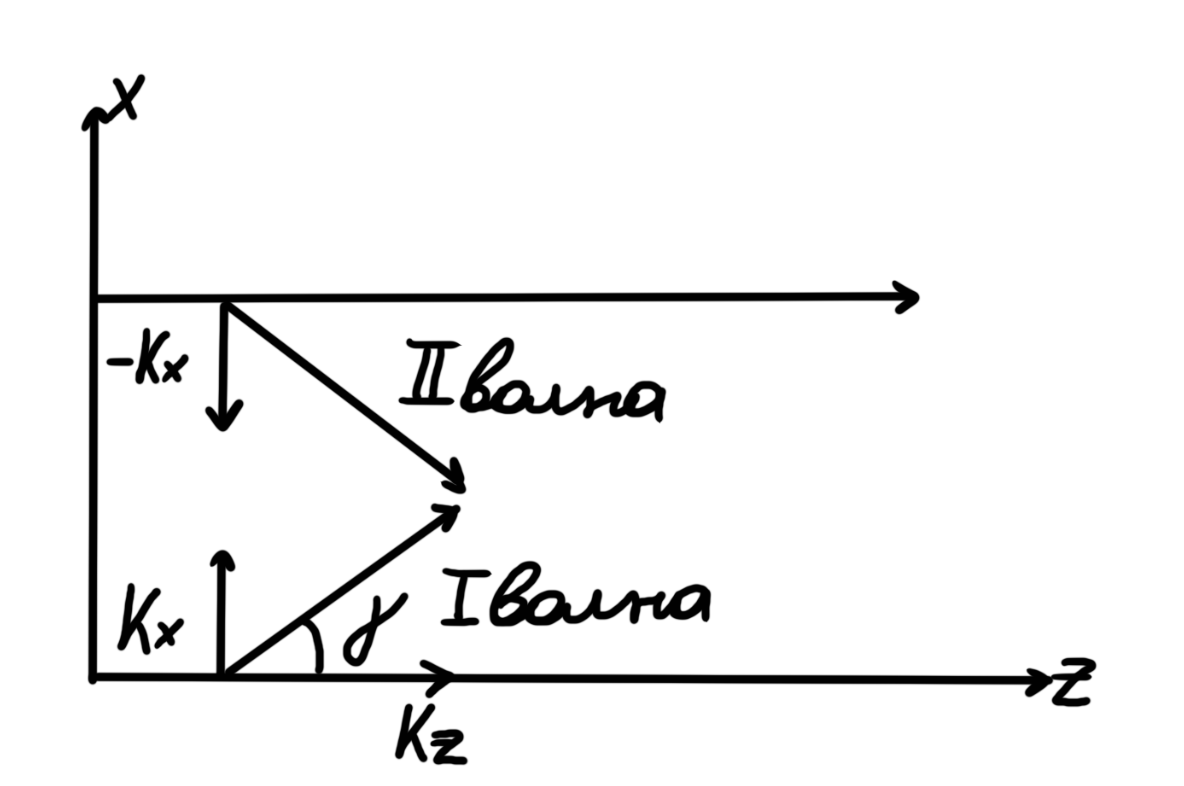
\includegraphics[width=0.4\textwidth]{/Users/vladbelousov/Desktop/Semestr_4-FP-NSU/ДфУ/Лекции_по_дням/image/57.png}
    \end{center}

    Возьмем \(\displaystyle  \varepsilon_0 = \min  \left\{   \varepsilon , \frac{r}{2 } \right\} \). Обозначим \(\displaystyle  m(\varepsilon_0) = \min_{\left\lVert \vec{y }  \right\rVert = \varepsilon_0 } V(\vec{y }  )>0  \) 

    \begin{center}
        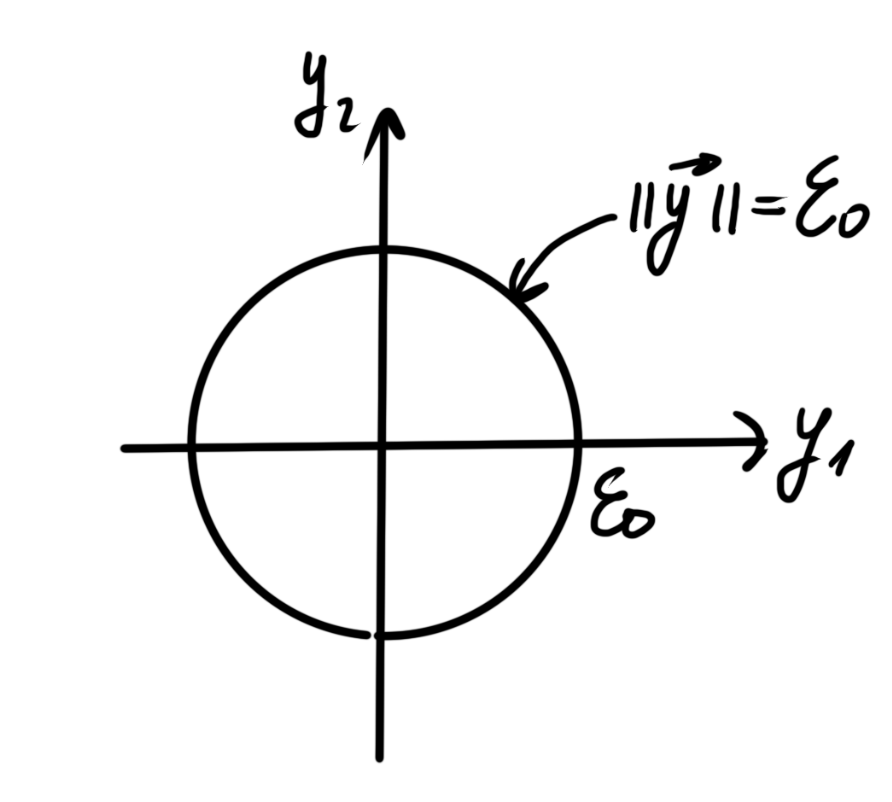
\includegraphics[width=0.4\textwidth]{/Users/vladbelousov/Desktop/Semestr_4-FP-NSU/ДфУ/Лекции_по_дням/image/58.png}
    \end{center}

    \[ M (\delta ) = \max _{\left\lVert \vec{y  }  \right\rVert \le  \delta } V(\vec{y }  )  \] 

    \begin{center}
        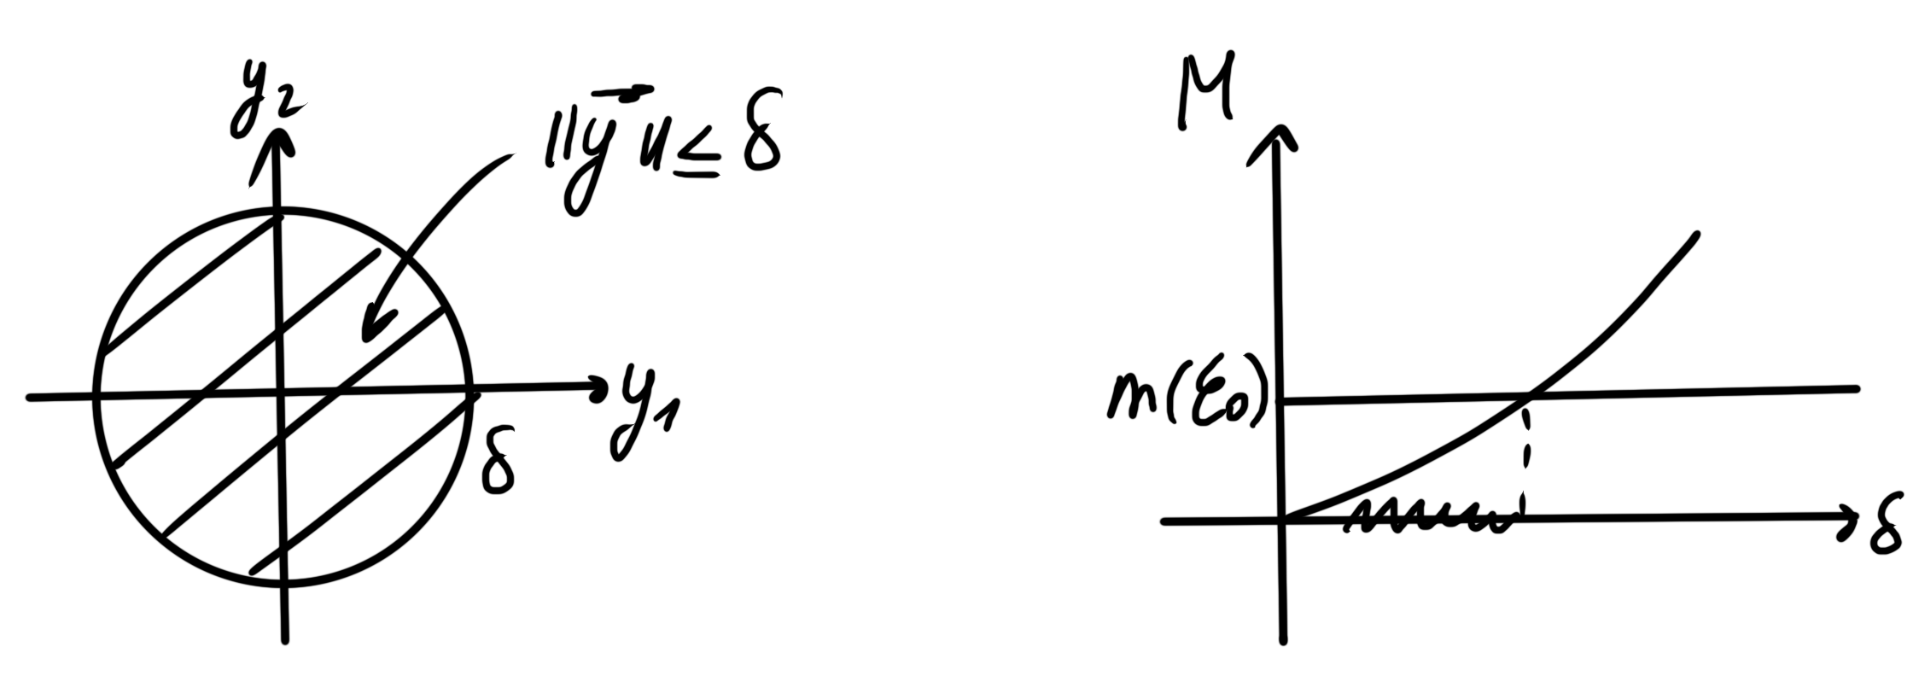
\includegraphics[width=0.7\textwidth]{/Users/vladbelousov/Desktop/Semestr_4-FP-NSU/ДфУ/Лекции_по_дням/image/59.png}
    \end{center}

    Выберем \( \delta  \) так, чтобы \( M(\delta ) < m (\varepsilon_0 ) \) 



    Утверждается, что \( \delta  < \varepsilon_0 \).

    От противного: пусть \( \delta \ge  \varepsilon_0  \). Тогда: 

    \[ m(\varepsilon_0 ) = \min _{\left\lVert \vec{y }  \right\rVert = \varepsilon_0} V(\vec{y } ) \le  \max _{ \left\lVert \vec{y }  \right\rVert = \varepsilon_0 }  V(\vec{y } ) \le  \max _{\left\lVert \vec{y }  \right\rVert \le  \varepsilon_0  } V(\vec{y} ) \overset{\delta \ge  \varepsilon_0}{\le } \max _{\left\lVert \vec{y }    \right\rVert \le  \delta } V(\vec{y }  ) = M(\delta )    \] 
    \begin{center}
        Противоречие \( \Rightarrow \delta < \varepsilon_0 \) \\
    \end{center} 

    Рассмотрим задачу Коши: 

    \[ \begin{aligned}
        \begin{cases}
            \displaystyle \frac{d}{dt }  \vec{y}  = \vec{f }  (\vec{y}  ) \\ 
            \vec{y } (t_0 ) = \vec{y }  _0
        \end{cases}
        \left\lVert \vec{y}  _0 \right\rVert <\delta 
    \end{aligned} \] 
    \( \Rightarrow \exists  !  \) непродолжаемое решение \( \vec{y}  (t ) \), определенное на открытом интервале \( \alpha , \omega ,\text{ }  t_0 \in  (\alpha , \omega ) , \text{  } \omega \le  + \infty  \) 

    Докажем, что \( \left\lVert \vec{y } (t) \right\rVert < \varepsilon_0 \text{ }  \forall   t \in [t_0 , \omega) \). 

    \begin{center}
        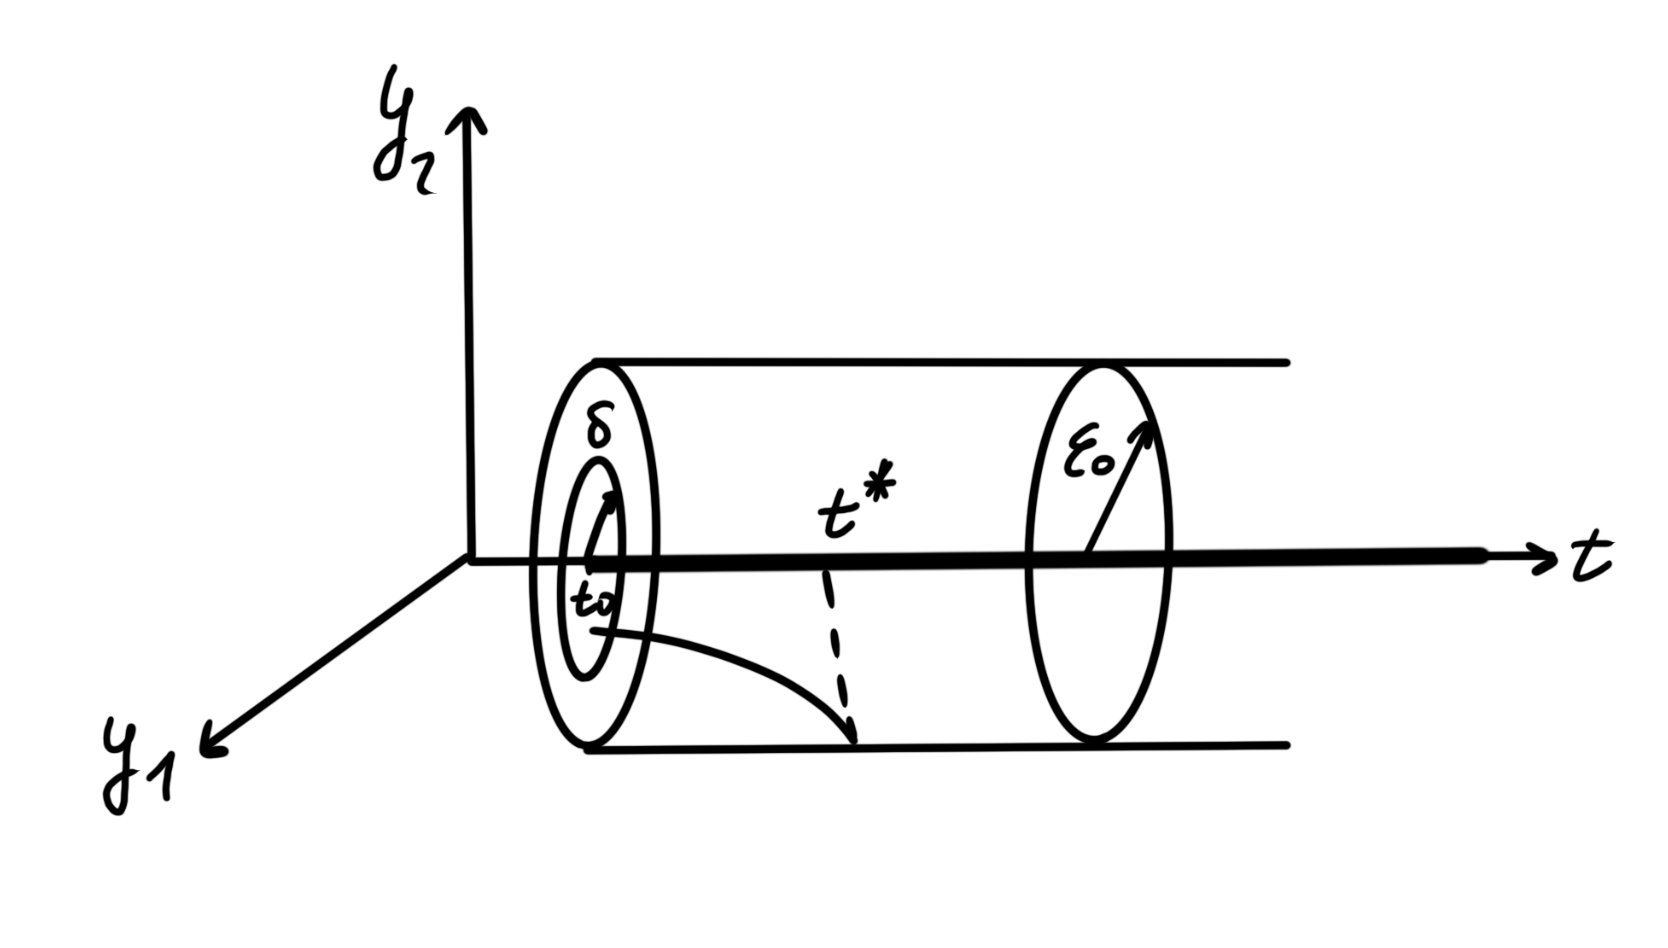
\includegraphics[width=0.7\textwidth]{/Users/vladbelousov/Desktop/Semestr_4-FP-NSU/ДфУ/Лекции_по_дням/image/60.png}
    \end{center}

    Пусть \( t^ * > t_0  \)  - первая точка, в которой \( \left\lVert \vec{y }  (t^* ) \right\rVert = \varepsilon_0 \), т.е \( \forall  t \in  [t_0,t^* ) : \left\lVert  \vec{y }  (t) \right\rVert < \varepsilon_0 \)  

    Воспользуемся условием 3) \( \nabla V (\vec{ y}  ) , \vec{f }  (\vec{y }  )  \le  0 , \text{ }  \left\lVert \vec{y }  \right\rVert < r\). 

    Возьмем решение \(\displaystyle  \vec{y}  (t ) , \text{ }  t \in  [t_0 , t^*] \Rightarrow \left\lVert \vec{y}  (t) \right\rVert \le  \varepsilon_0 \le \varepsilon_0 = \min \left\{   \varepsilon , \frac{r}{2 } \right\} \le  \frac{r}{2 }  <r \) 

    Возьмем \(\displaystyle  V (\vec{y }  (t ) ) \Rightarrow   \) 
    \[ \Rightarrow\frac{d}{dt }  V(\vec{y}  (t ) ) = \frac{d}{dt }  V (y_1(t ),..., y_n (t)) = \frac{\partial  V }{\partial  y_1 } (\vec{y}  (t ) )\underbrace{ \frac{d y_1(t )}{ dt }}_{f_1 (\vec{y} )}+ ...+ \frac{\partial  V }{\partial  y_n } (\vec{y }  (t )) \underbrace{\frac{d y_n(t )}{dt} }_{f_n (\vec{y} ) } =      \] 
    \[ = ( \nabla  V(\vec{y} (t )) , \vec{f }  (\vec{y}  (t ))) \le  0 \] 
 
    Получили \( \displaystyle  \frac{d}{dt }  V(\vec{y} (t )) \le  0 , \text{ }  t \in  [ t_0 , t^*] \)  


    \[ V(\vec{y}  (t ^* )) \le  V (\vec{y}  (t_0)) \tag{\(*  \) }\] 
    \[ V(\vec{y}  (t^* )) \ge  \min _{\left\lVert \vec{y}  \right\rVert = \varepsilon_0} V (\vec{y } ) = m(\varepsilon_0 )    \tag{\(**  \) }     \] 
    \[ V(\vec{y}  (t_0 ) )= V(\vec{y} _0  ) \le  \max _{\left\lVert \vec{y}  \right\rVert \le  \delta } V(\vec{y}  ) = M(\delta )  \tag{\(*  **\) } \] 

    \[ m(\varepsilon_0 ) \overset{(**)}{\le}  V(\vec{y }  (t^*)) \overset{(*)}{\le}  V(\vec{y }  (t_0)) \overset{(***)}{\le}  M(\delta )\text{ - противоречие.}  \] 
    \[ \Rightarrow \left\lVert \vec{y } (t) \right\rVert < \varepsilon_0 \text{  }  \forall  r \in  [ t_0 , \omega) \] 

    Мы доказали: 
    \[ \forall  \varepsilon > 0 \text{ }  \exists  \delta > 0 : \left\lVert \vec{y} (t_0) \right\rVert < \delta \Rightarrow \left\lVert \vec{y}  (t) \right\rVert < \varepsilon \text{ } \forall  r \in  [t_0 , \omega) \] 

    \begin{center}
        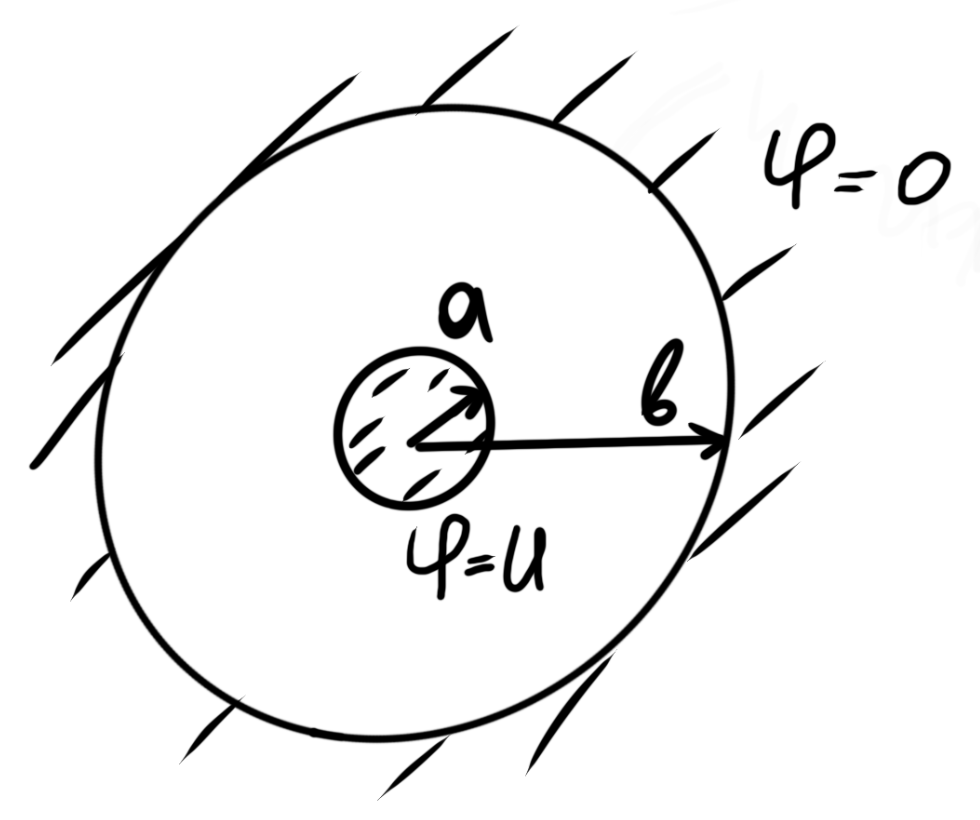
\includegraphics[width=0.7\textwidth]{/Users/vladbelousov/Desktop/Semestr_4-FP-NSU/ДфУ/Лекции_по_дням/image/61.png}
    \end{center}

    Пусть \( \omega < + \infty  , \text{  } \displaystyle  \lim_{t  \to \omega- 0} \vec{y } (t ) = \vec{y}  _{ \omega } \in  \mathbb{R} ^n    \) 

    Рассмотрим задачу Коши: 

    \[ \begin{aligned}
    \begin{cases}
        \displaystyle \frac{d}{dt }  \vec{y } = \vec{f }  (\vec{y }  ) \\
        \vec{y } (\omega ) = \vec{y } _{\omega} 
    \end{cases}
    \end{aligned} \] 
    \( \Rightarrow  \) по теореме Пикара \( \exists !  \) непродолжаемое решение \( \tilde{t } (t ) , \text{  }  t \in  (\tilde{\alpha } ,\tilde{ \omega }) , \text{ } \omega \in  (\tilde{ \alpha } , \tilde{ \omega})  \) 

    Рассмотрим функцию: 

    \[ \begin{aligned}
        z(t )=
     \begin{cases}
     y(t ) , \text{ }  t \in  [t_0 , \omega) \\
     \tilde{y } (t ) ,\text{ }  t \in  [\omega , \tilde{\omega})
     \end{cases}
     \text{  - продолжаемое решения }   y(t) \text{, т.е решение задачи Коши} 
    \end{aligned} \]  


\[ \begin{cases}
    \displaystyle  \frac{d}{dt }  \vec{y}  = \vec{f }  (\vec{y}  ) \\ 
    \vec{y }  (t_0 ) = \vec{y}  _0
    \end{cases} \] 
    
    Почему \( \displaystyle  \exists  \frac{d}{dt }  z(t ) \bigg | _{ t = \omega } ?   \) 
    
    \[ \frac{d}{dt }  z(t ) \bigg | _{t = \omega  -0 }  = \vec{f }  (\vec{y } ) | _{t = \omega - 0 } = \vec{f }  (\vec{y } _{\omega} )   \] 
    \[ \frac{d}{dt }  z(t ) \bigg | _{t = \omega  +0 }  = \vec{f }  (\vec{y } ) | _{t = \omega +0 } = \vec{f }  (\vec{y } _{\omega} )   \] 
    
    Противоречие с тем, что \( \vec{y } (t) \) - непродолжаемое решение \( \Rightarrow \omega = + \infty  \Rightarrow  \) доказан пункт 3). 
    
    
    2) Возьмем \( \displaystyle  \varepsilon = \frac{r ' }{2 } \Rightarrow \exists  \delta \left(  \frac{r}{2 }  \right) \Rightarrow  \Delta  = \delta \left( \frac{r}{2 }  \right) \Rightarrow  \) доказан пункт 2). 
    
    \[  \Rightarrow \vec{y } ^* (t ) = 0  \text{ устойчиво по Ляпунову} \] 
\end{proof}

\begin{theorem}[Теорема Ляпунова об асимптотической устойчивости] 
    Пусть функция \( V(\vec{y} ) \)  такая, что выполнено условие 1), 2), \( 3^*) (\nabla V (\vec{y }  ,\vec{f }  (\vec{y } ))) < 0  ,\text{ }  0 < \left\lVert  \vec{y }  \right\rVert < r  \). Тогда \( \vec{y } ^* (t ) = 0 \) системы (1) асимптотически устойчиво.

    Без доказательства.
\end{theorem}

\begin{theorem}[Теорема Ляпунова о неустойчивости]
    Пусть существует функция \( V(\vec{y } ) \), удовлетворяющее условиям 1), 2),  \(3^{** } ) (\nabla V (\vec{y}  ) \vec{f } (\vec{y } ) ) >0 , \text{ }  0 < \left\lVert \vec{y }  \right\rVert < r  \). Тогда \( \vec{y } ^* (t ) = 0 \)   неустойчиво. 
\end{theorem}

\begin{proof} \(  \) 

    От противного: пусть \( \vec{y } ^* (t)  = 0 \) устойчиво по Ляпунову, в частности, \( \forall  \varepsilon > 0 \text{ }  \exists  \delta > 0  \text{ }  \forall  \vec{y } (t_0 ) : \left\lVert  \vec{y}  (t_0 ) \right\rVert < \delta \Rightarrow \left\lVert \vec{y}  (t) \right\rVert < \varepsilon \text{ } \forall  t > t_0 \) 

    Возьмем \( \displaystyle  \varepsilon = \frac{r}{2 }  \Rightarrow \exists  \delta \left( \frac{r}{2 }    \right) : \left\lVert \vec{y} (t_0 ) \right\rVert < \delta \left( \frac{r}{2}  \right) \Rightarrow \left\lVert \vec{y} (t ) \right\rVert < \frac{r}{2 }  <r  \text{ }  \forall  t \ge  t_0 \) 

    \begin{center}
        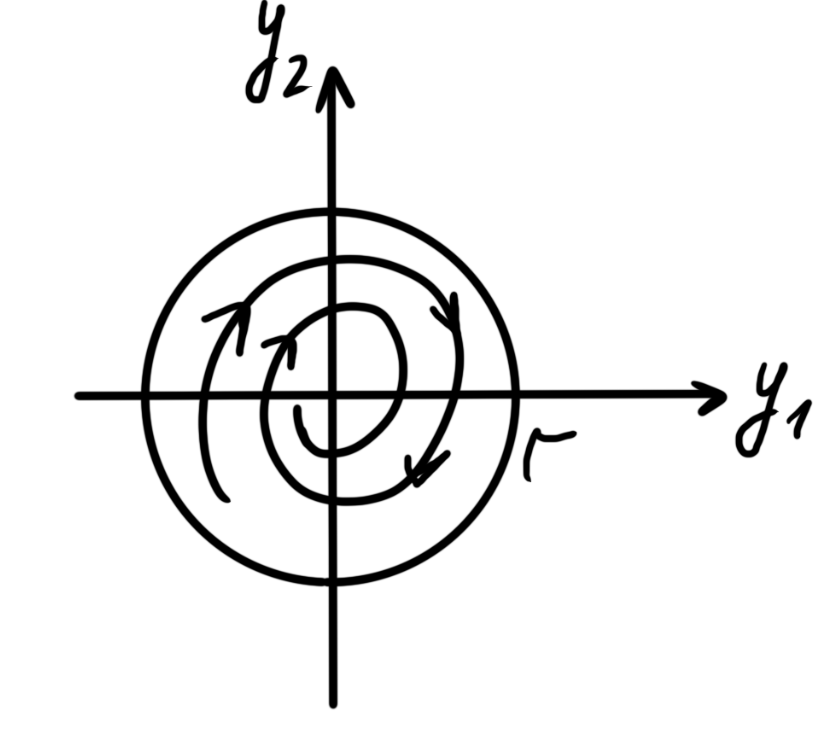
\includegraphics[width=0.4\textwidth]{/Users/vladbelousov/Desktop/Semestr_4-FP-NSU/ДфУ/Лекции_по_дням/image/62.png}
    \end{center}

    Рассмотрим задачу Коши: 

    \[\begin{aligned}
        \begin{cases}
            \displaystyle \frac{d}{dt } \vec{y}  = \vec{f } (\vec{y} ) \\
            \vec{y } (t_0) = \vec{y } _0
        \end{cases} 
        , \left\lVert \vec{y}  _0 \right\rVert < \delta \left( \frac{r}{2 }  \right) , \text{ }  \kern-0.8cm\underbrace{\vec{y } _0}_{\vec{y}  (t ) \neq 0 ,\text{ }  \forall  t \ge  t_0} \kern-0.8cm \neq \vec{0} \Rightarrow  \left\lVert \vec{ y } (t ) \right\rVert < \frac{r}{2 }  \text{ }  \forall  t \in  [ t_0 , + \infty ) 
    \end{aligned}\] 

    \begin{center}
        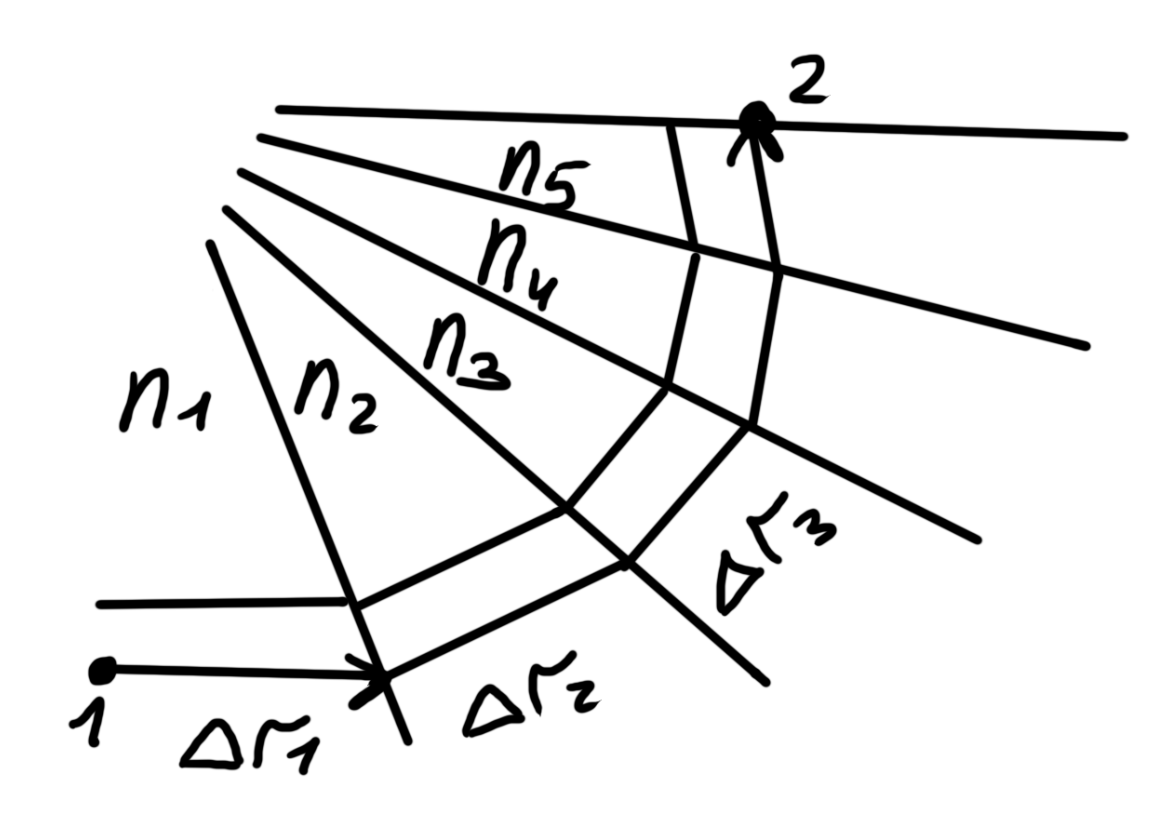
\includegraphics[width=0.7\textwidth]{/Users/vladbelousov/Desktop/Semestr_4-FP-NSU/ДфУ/Лекции_по_дням/image/63.png}
    \end{center}

    \[ \begin{aligned}
    \begin{cases}
    \displaystyle  \frac{d}{dt }  \vec{y}  = \vec{f } (\vec{y} ) \\ 
    \vec{y } (\tilde{t } ) = 0
    \end{cases}
    \Rightarrow \vec{y } ^* (t ) = 0 \text{ - решение.} 
    \end{aligned} \] 


\( 3) \Rightarrow \displaystyle  \frac{d}{dt }  V(\vec{y}  (t))  = (\nabla V(\vec{y }  (t ) ) , \vec{f }  (\vec{y}(t) )) > 0 ,\text{ }  t \ge  t_0 \) 

\[ V(\vec{y } (t )) > \underbrace{V (\vec{y } (t_0))}_{= \alpha > 0} ,\text{ } t> t_0 \] 
\[ V(\vec{y}  (t) ) > \alpha , \text{ }  t \ge  t_0 \] 

Рассмотрим множество \( \displaystyle  \underbrace{\left\{   \vec{ y}  : \mathbb{R} ^2 : \left\lVert \vec{y}  \right\rVert \le  \frac{r}{2 }  , \text{ }  V(\vec{y } ) \ge  \alpha \right\}}_{P}\)- компакт, \( \forall  t \ge  t_0 , \text{ }  \left\lVert \vec{y}(t)  \right\rVert \in  P , \text{ } \vec{0 }\text{ }  \cancel{\in  } \text{ } P\)  

Рассмотрим: 

\[ \min_{\vec{y } \in  P } (\nabla V (\vec{y}  ) , \vec{f } (\vec{y} )) = \gamma > 0   \] 
\[ \frac{d}{dt  } V(\vec{y }(t)  ) = (\nabla V(\vec{y} (t)) , \vec{f }  (\vec{y } (t)))\overset{\vec{y} (t) \in  P}{ \ge}  \gamma > 0 \text{ }  \bigg | \int_{t_0}^{t}     \] 
\[ \int_{t_0}^{t } \frac{d}{ds }  V(\vec{y} (s )) ds \ge  \int_{t_0}^{t } \gamma ds    \] 
\[ V(\vec{y } (t )) \ge  V(\vec{y } (t_0)) + \underbrace{\gamma (t -t_0 )}_{\to  \infty } , \text{ }  \forall  t \ge  t_0 \text{ при } t \to  +\infty \] 
\[ \Rightarrow V(\vec{y} (t)) \to  \infty  \] 

\[ \left\lVert  \vec{y} (t) \right\rVert \le  \frac{r}{2 }  \] 
\[ V(\vec{y} (t )) \le  \max _{\left\lVert  \vec{y}  \right\rVert \le  \frac{r}{2 } } V(\vec{y} ) < + \infty   \] 
\[ \text{Противоречие.}  \] 

\[ \Rightarrow \vec{y } ^* (t ) = 0  \text{ неустойчиво } \] 

\end{proof}

Пример: Исследовать на устойчивость нулевое решение: 

\[ \begin{aligned}
    \begin{cases}
        y_1 ' =y_2 + \alpha y_1 ^3  \\ 
        y_2 ' = -y_1 \alpha y_2 ^3
    \end{cases} 
    \begin{cases}
    y_1^* (t ) = 0 \\
    y_2^* (t ) = 0
    \end{cases}
    \text{ - решение.} 
\end{aligned}\] 


\[ V(y_1,y_2 ) = a y_1 ^{2n }  + b y_2 ^{2 m }  \text{ }  (a,b > 0 \text{ }  m  , n \in \mathbb{N}) -\text{ выполнены } 1),2) \] 
, где \( a , b > 0 , \text{ }  n , m \in  \mathbb{N} \) 

\[ (\nabla V ,f )  = \left( \begin{pmatrix}
2a  n y^{2n -1 }_1 \\
2b  m y^{2m - 1 }  _2 
\end{pmatrix} , \begin{pmatrix}
y_2 + \alpha y_1 ^3 \\
-y_1+ \alpha y_2 ^3
\end{pmatrix}\right) =  \]  
\[ =2n a y_1 ^{2n -1 }  y_2 + 2n a y_1 ^{2n -1 }  \alpha y_1 ^3  + 2 bm y_2 ^{2m - 1 }  +2 m b y^{2 m- 1 } y_2 ^3\] 




%%-------------------------------%%

% Закрытие документа, если файл компилируется отдельно
\ifdefined\mainfile
    % Если это основной файл, не нужно заканчивать документ
\else
    \end{document}
\fi